% Content for Chapter 5, Section 5.1 — pulled in by chapters/05-system-design.tex
\subsection{لمحة عن دور كل خدمة}

يتألّف النظام من ستّ خدمات مصغّرة مستقلّة تعمل خلف بوّابة واحدة (\en{Gateway}). وتتشارك هذه الخدمات بنيةً تحتية تضمّ قواعد بيانات منفصلة وناقل رسائل (\en{Message Bus}) ومخزن ملفّات وخادم وسائط. وفيما يأتي دور كل خدمة منها:

\begin{enumerate}
  \item \textbf{خدمة إدارة المستخدمين} (\en{UserManagementService}): تتولّى الهوية والأدوار والصلاحيات. وتقوم بإصدار رموز الوصول، وتدير التسجيل والدخول واستعادة كلمة المرور، وتنفّذ العمليات الإدارية التي تمسّ بقيّة الخدمات.
  \item \textbf{خدمة الفصول الدراسية} (\en{ClassroomService}): تدير الفصول والعضوية والجلسات والاختبارات والملفّات المرجعية، إضافةً إلى مخرجات الجلسات من تسجيلات وملخّصات.
  \item \textbf{خدمة البث} (\en{StreamingService}): تدير غرف البث المباشر وصلاحيات النشر فيها، وتتولّى تسجيل الجلسات عبر \en{LiveKit Egress} وحفظها في مخزن الملفّات.
  \item \textbf{خدمة البريد} (\en{EmailService}): تتلقّى الرسائل من الناقل وترسل الإشعارات البريدية المقابلة لها.
  \item \textbf{خدمة المعرفة} (\en{RagService}): تحوّل المواد المرجعية إلى مقاطع (\en{Chunks}) قابلة للبحث الدلالي، وتخدم الاسترجاع، وتولّد ملخّصات الجلسات.
  \item \textbf{خدمة المساعد المباشر} (\en{LiveAssistantService}): تحوّل كلام الجلسة الجارية إلى نص، وتقيّم محتواه مقابل المصادر المفهرسة، وتقدّم مساعدة تعليمية مباشرة للمعلّم في أثناء الشرح.
\end{enumerate}

\subsection{مخطط مكوّنات النظام}

يعرض الشكل~\ref{fig:arch-01} هذه الخدمات مجتمعةً مع البنية التحتية والبوّابة وتطبيق الويب.

\begin{figure}[htbp]
  \centering
  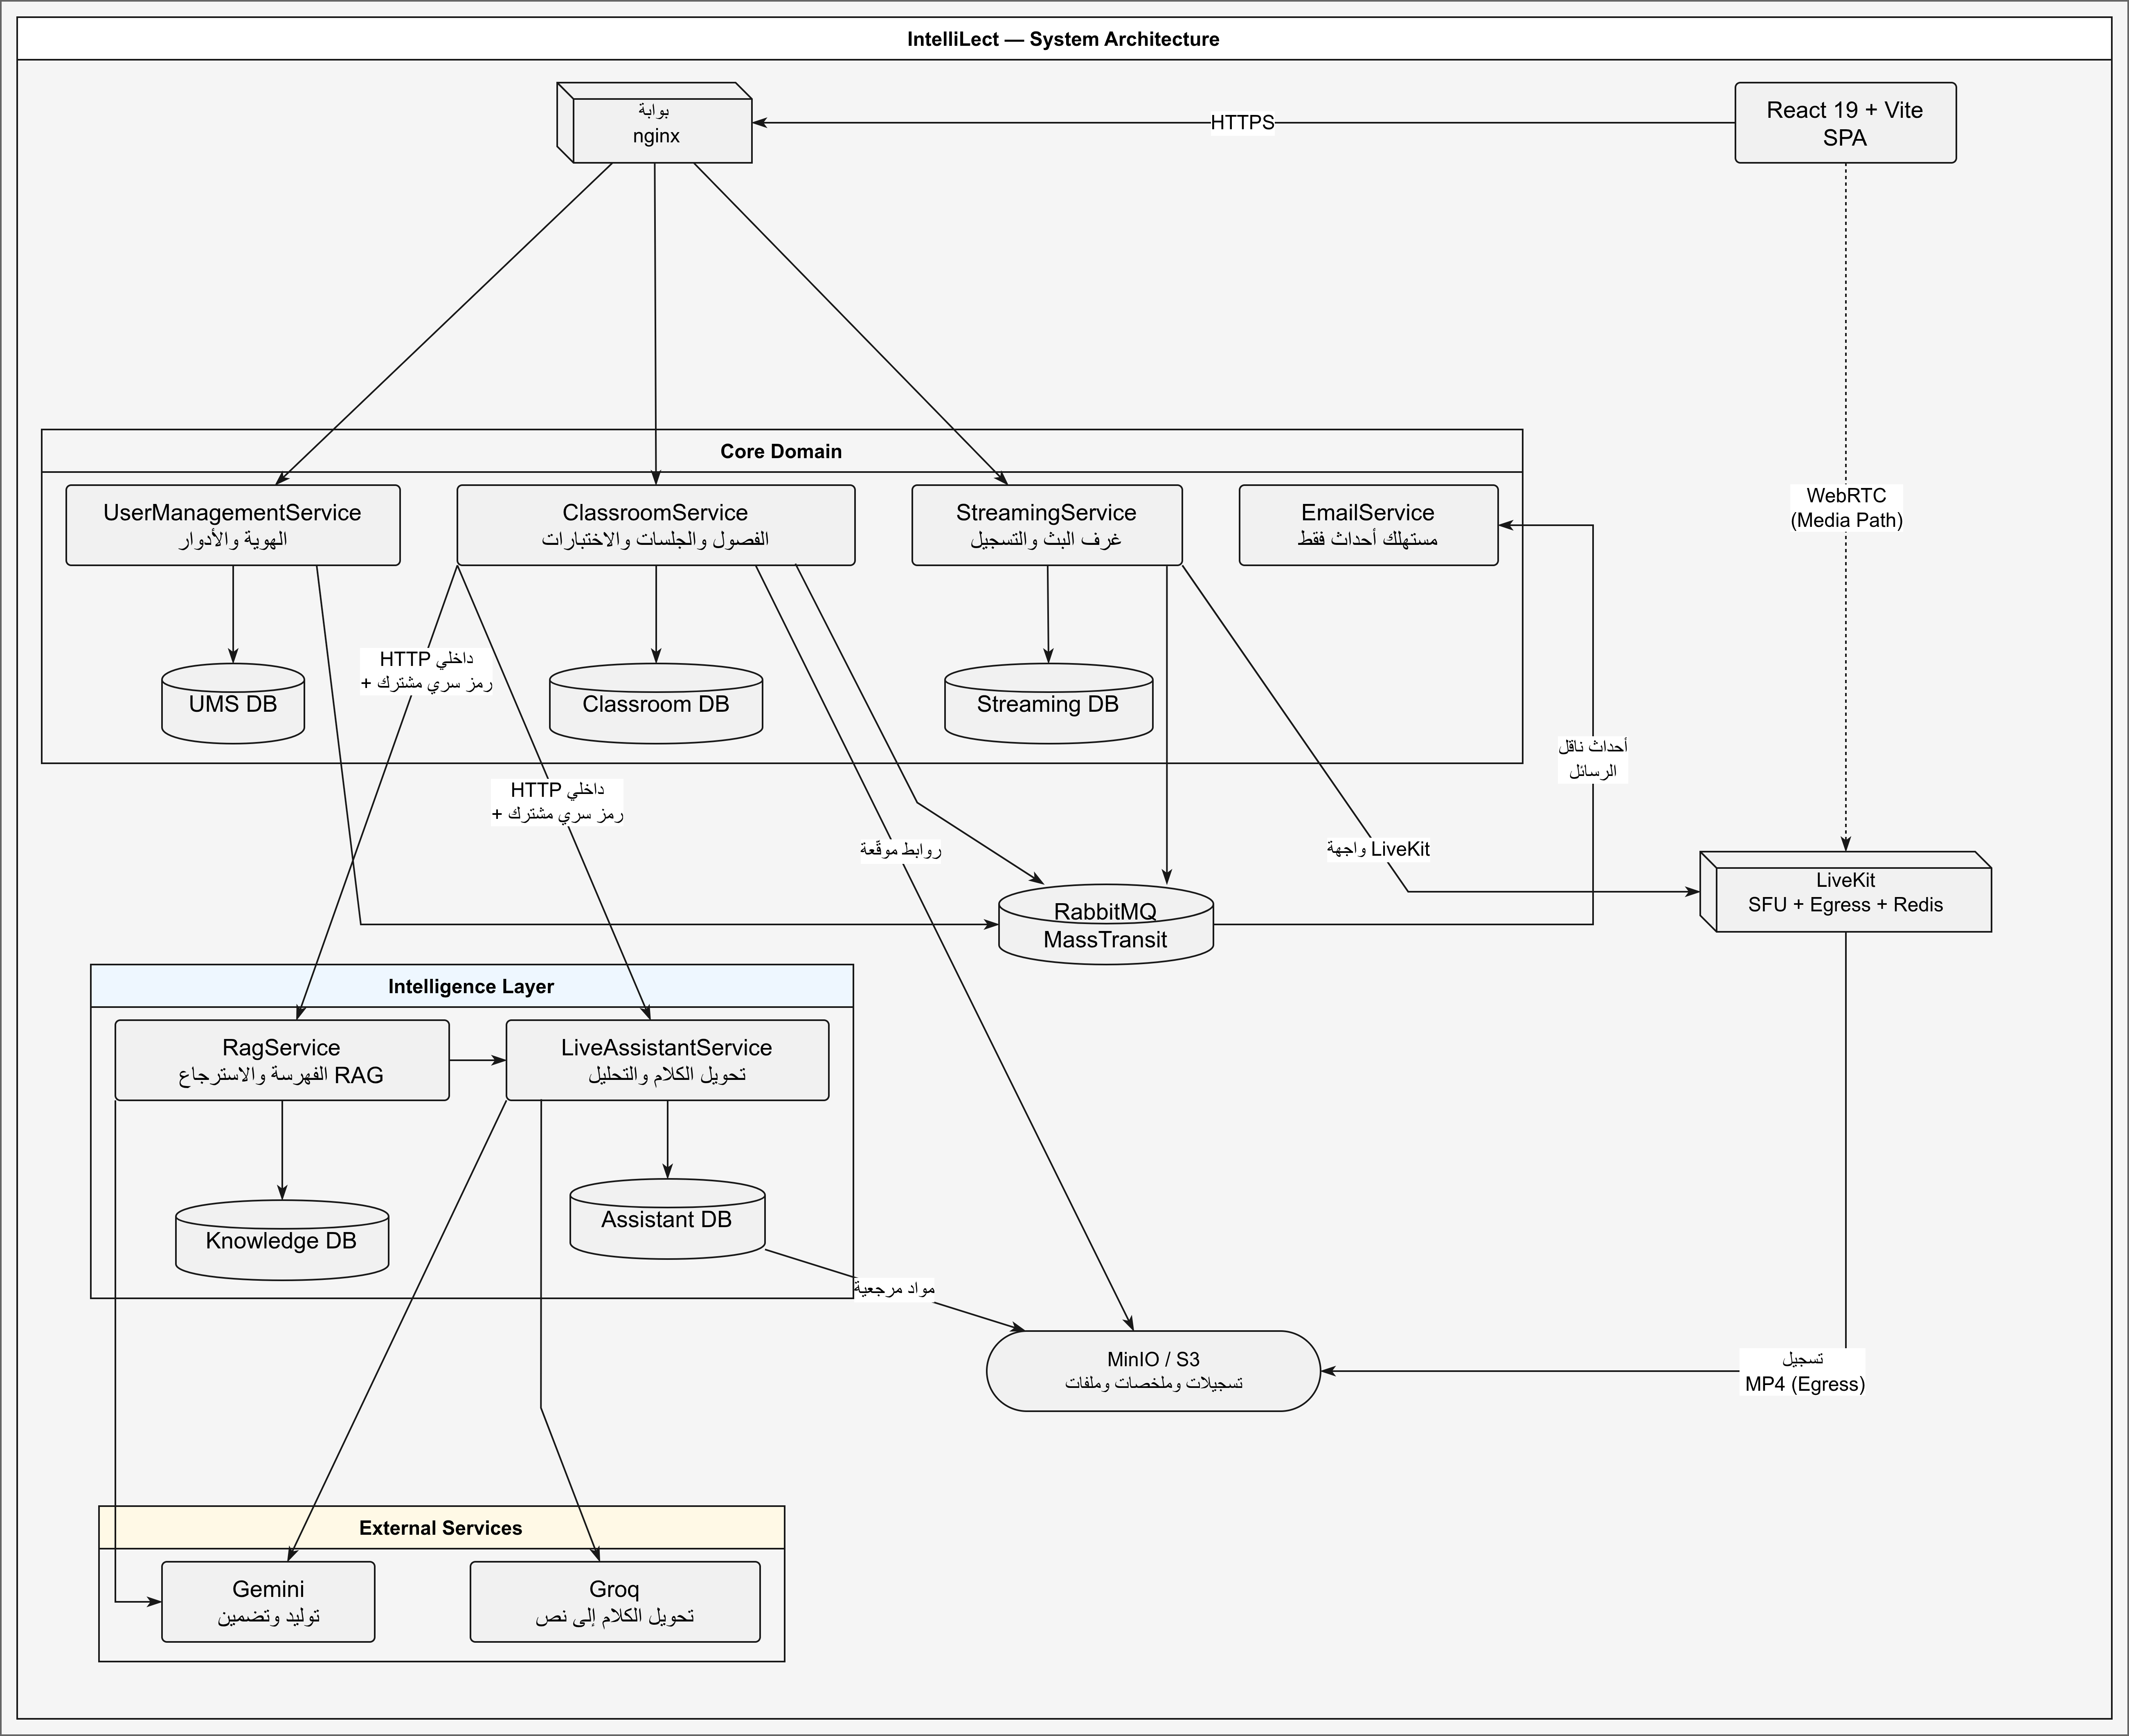
\includegraphics[width=\textwidth,height=0.8\textheight,keepaspectratio]{figures/arch-01-system-block.png}
  \caption{مخطط المكوّنات العام للنظام.}
  \label{fig:arch-01}
\end{figure}


\subsection{نمطا الاتصال بين الخدمات}

يقوم الاتصال بين الخدمات على نمطين أساسيين:

\begin{enumerate}
  \item \textbf{اتصال مباشر (متزامن) عبر \en{HTTP}}: يُستعمل حين تحتاج الخدمة إلى جواب قبل إكمال عملها. وتُعرَض هذه النقاط تحت المسار \en{/api/internal}، ولا تمرّ عبر البوّابة، ويحرسها سرٌّ مشترك يُرسَل في الترويسة \en{X-Internal-Secret}.
  \item \textbf{اتصال غير مباشر (غير متزامن) عبر ناقل الرسائل}: يُستعمل حين لا تحتاج الخدمة المرسِلة إلى جواب. ويُنفَّذ هذا النمط بالناقل \en{RabbitMQ} بوساطة \en{MassTransit}.
\end{enumerate}
